\chapter{Datasets}


We evaluated the quality of our models' representations with music classification experiments. We used the MagnaTagATune \cite{law2009evaluation} dataset and Million Song Dataset \cite{Bertin-Mahieux2011} for pre-training and evaluation. For the transfer learning experiments, we pre-train on the Million Song, fault-filtered GTZAN \cite{tzanetakis2002musical,sturm2013gtzan}, McGill Billboard \cite{burgoyne_billboard} and Free Music Archive \cite{fma_dataset} datasets and subsequently perform evaluation on the MagnaTagATune dataset. 

Predicting the top~50 tags in the Magna\-Tag\-A\-Tune and Million Song datasets are a popular benchmark for music classification. It is a multi-label classification task: each track can have multiple tags, of which we use the 50 most frequently occuring to compare our performance against supervised benchmarks. 
For the Magna\-Tag\-A\-Tune dataset, we used the original, MIREX 2009 version, consisting of 25\,863 songs, and the same dataset split, so that we can compare our results with previous work easily \cite{pons_end--end_2017, lee2018samplecnn, dieleman_feature_learning}. It should be noted that this original version contains tag labels that are synonymous, e.g., `female', `woman', `no vocal', `no voice' and also contains tracks with no labels. The tags for the Million Song Dataset are less overlapping, and contain more semantic tags, e.g., `beautiful', `happy' and `sad' which are arguably harder to linearly separate during the linear evaluation phase.
Like other studies, we use average tag-wise ROC-AUC and PR-AUC scores as evaluation metrics, which are global measures indicating how well the classifier ranks segments given a tag. PR-AUC is calculated in addition to ROC-AUC because ROC-AUC scores can be over-optimistic for imbalanced datasets like Magna\-Tag\-A\-Tune\cite{pons_end--end_2017}. 

From the McGill Billboard dataset, we use 461 audio files of contemporary pop songs for training. While this dataset is most often used for evaluating chord recognition algorithms, we use it solely for self-supervised pre-training.
Similarly, we use the Free Music Archive dataset, consisting of 22\,413 unique multi-labeled songs for the `medium' version, and the fault-filtered GTZAN dataset containing 930 segments of 30 seconds, each having a single label denoting its genre.


\section{MagnaTagATune}

\begin{figure}[t]
    \centering
    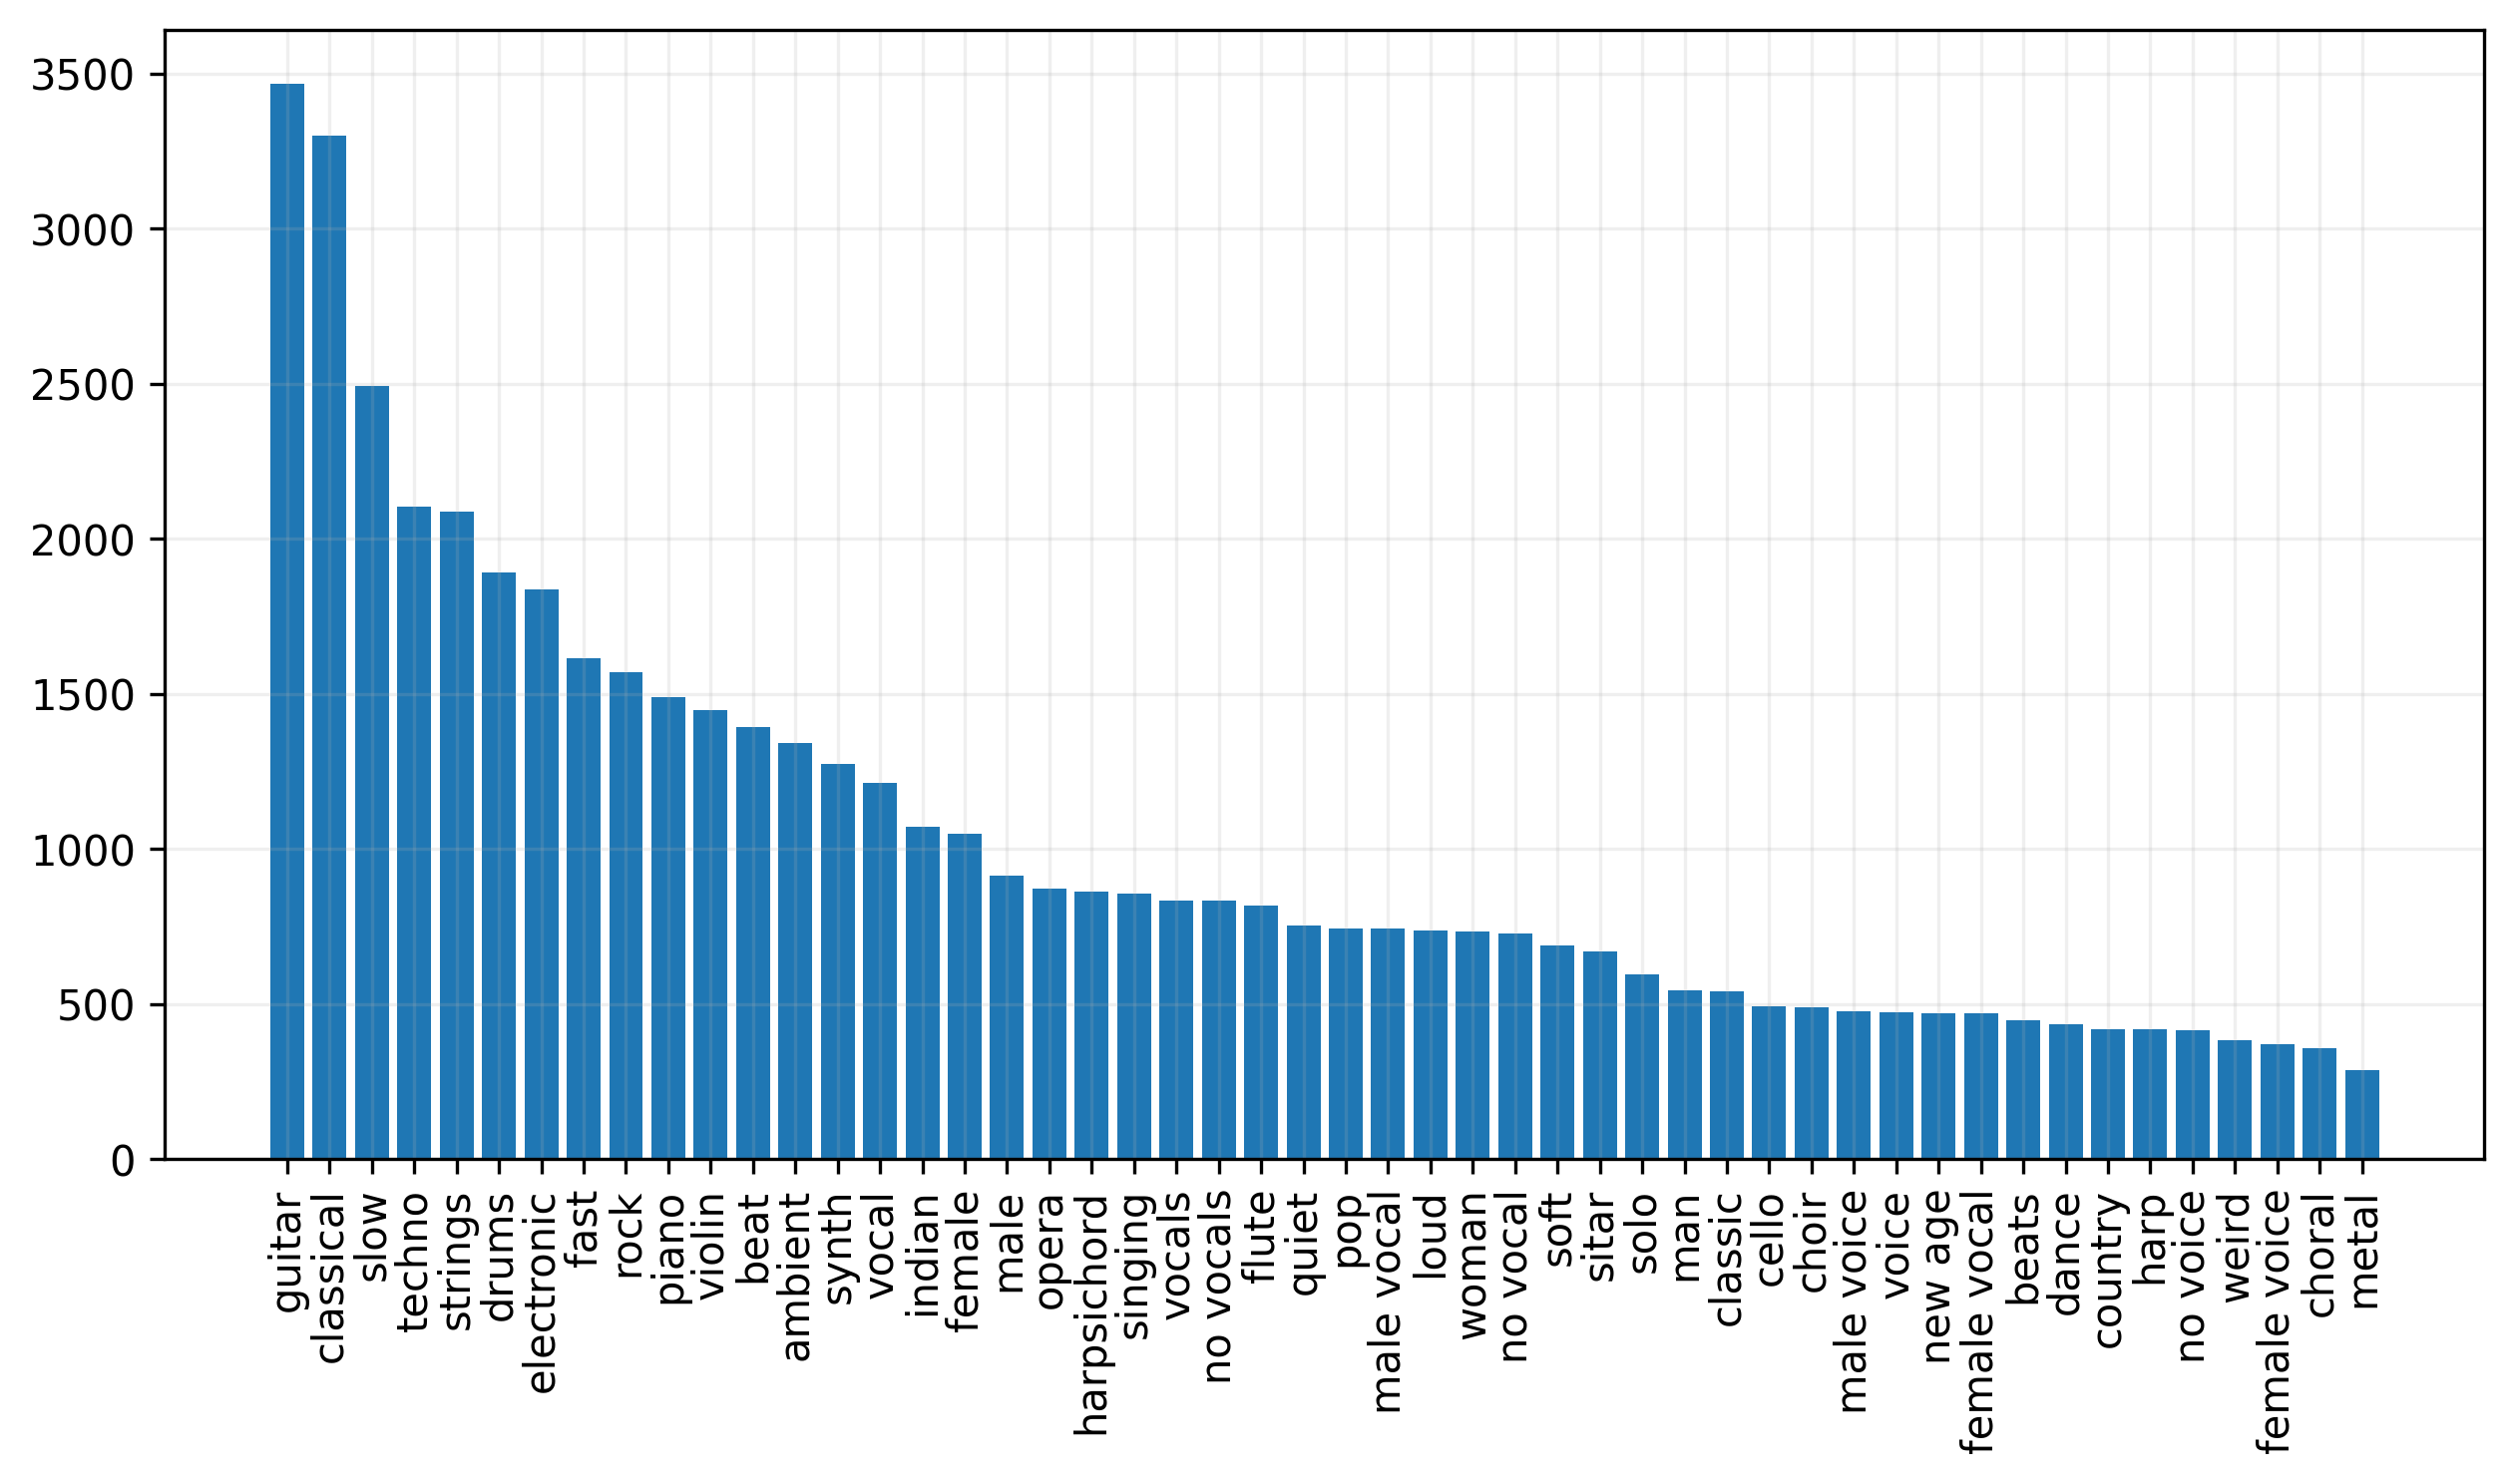
\includegraphics[width=\columnwidth]{figs/tag_stats_magnatagatune.png}
    \caption{Distribution of tags of the MagnaTagATune dataset}
    \label{fig:tag_stats_magnatagatune}
\end{figure}


\begin{table}[t]
    \centering
    \begin{tabular}{lll}\toprule
        guitar  & classical & slow \\
        techno & strings & drums \\
        electronic & rock & fast \\
        piano & ambient & beat \\
        violin & vocal & synth \\
        female & indian & opera \\
        male & singing & vocals \\
        no vocals & harpsichord & loud \\
        quiet & flute & woman \\
        male vocal & no vocal & pop \\
        soft & sitar & solo \\
        man & classic & choir \\
        voice & new age & dance \\
        male voice & female vocal & beats \\
        harp & cello & no voice \\
        weird & country & metal \\
        female voice & choral & - \\                 
        \bottomrule
    \end{tabular}
    \caption{50 most popular tags in the MagnaTagATune dataset}
    \label{tab:magnatagatune_tags}
\end{table}





\section{Million Song Dataset}

\begin{figure}[t]
    \centering
    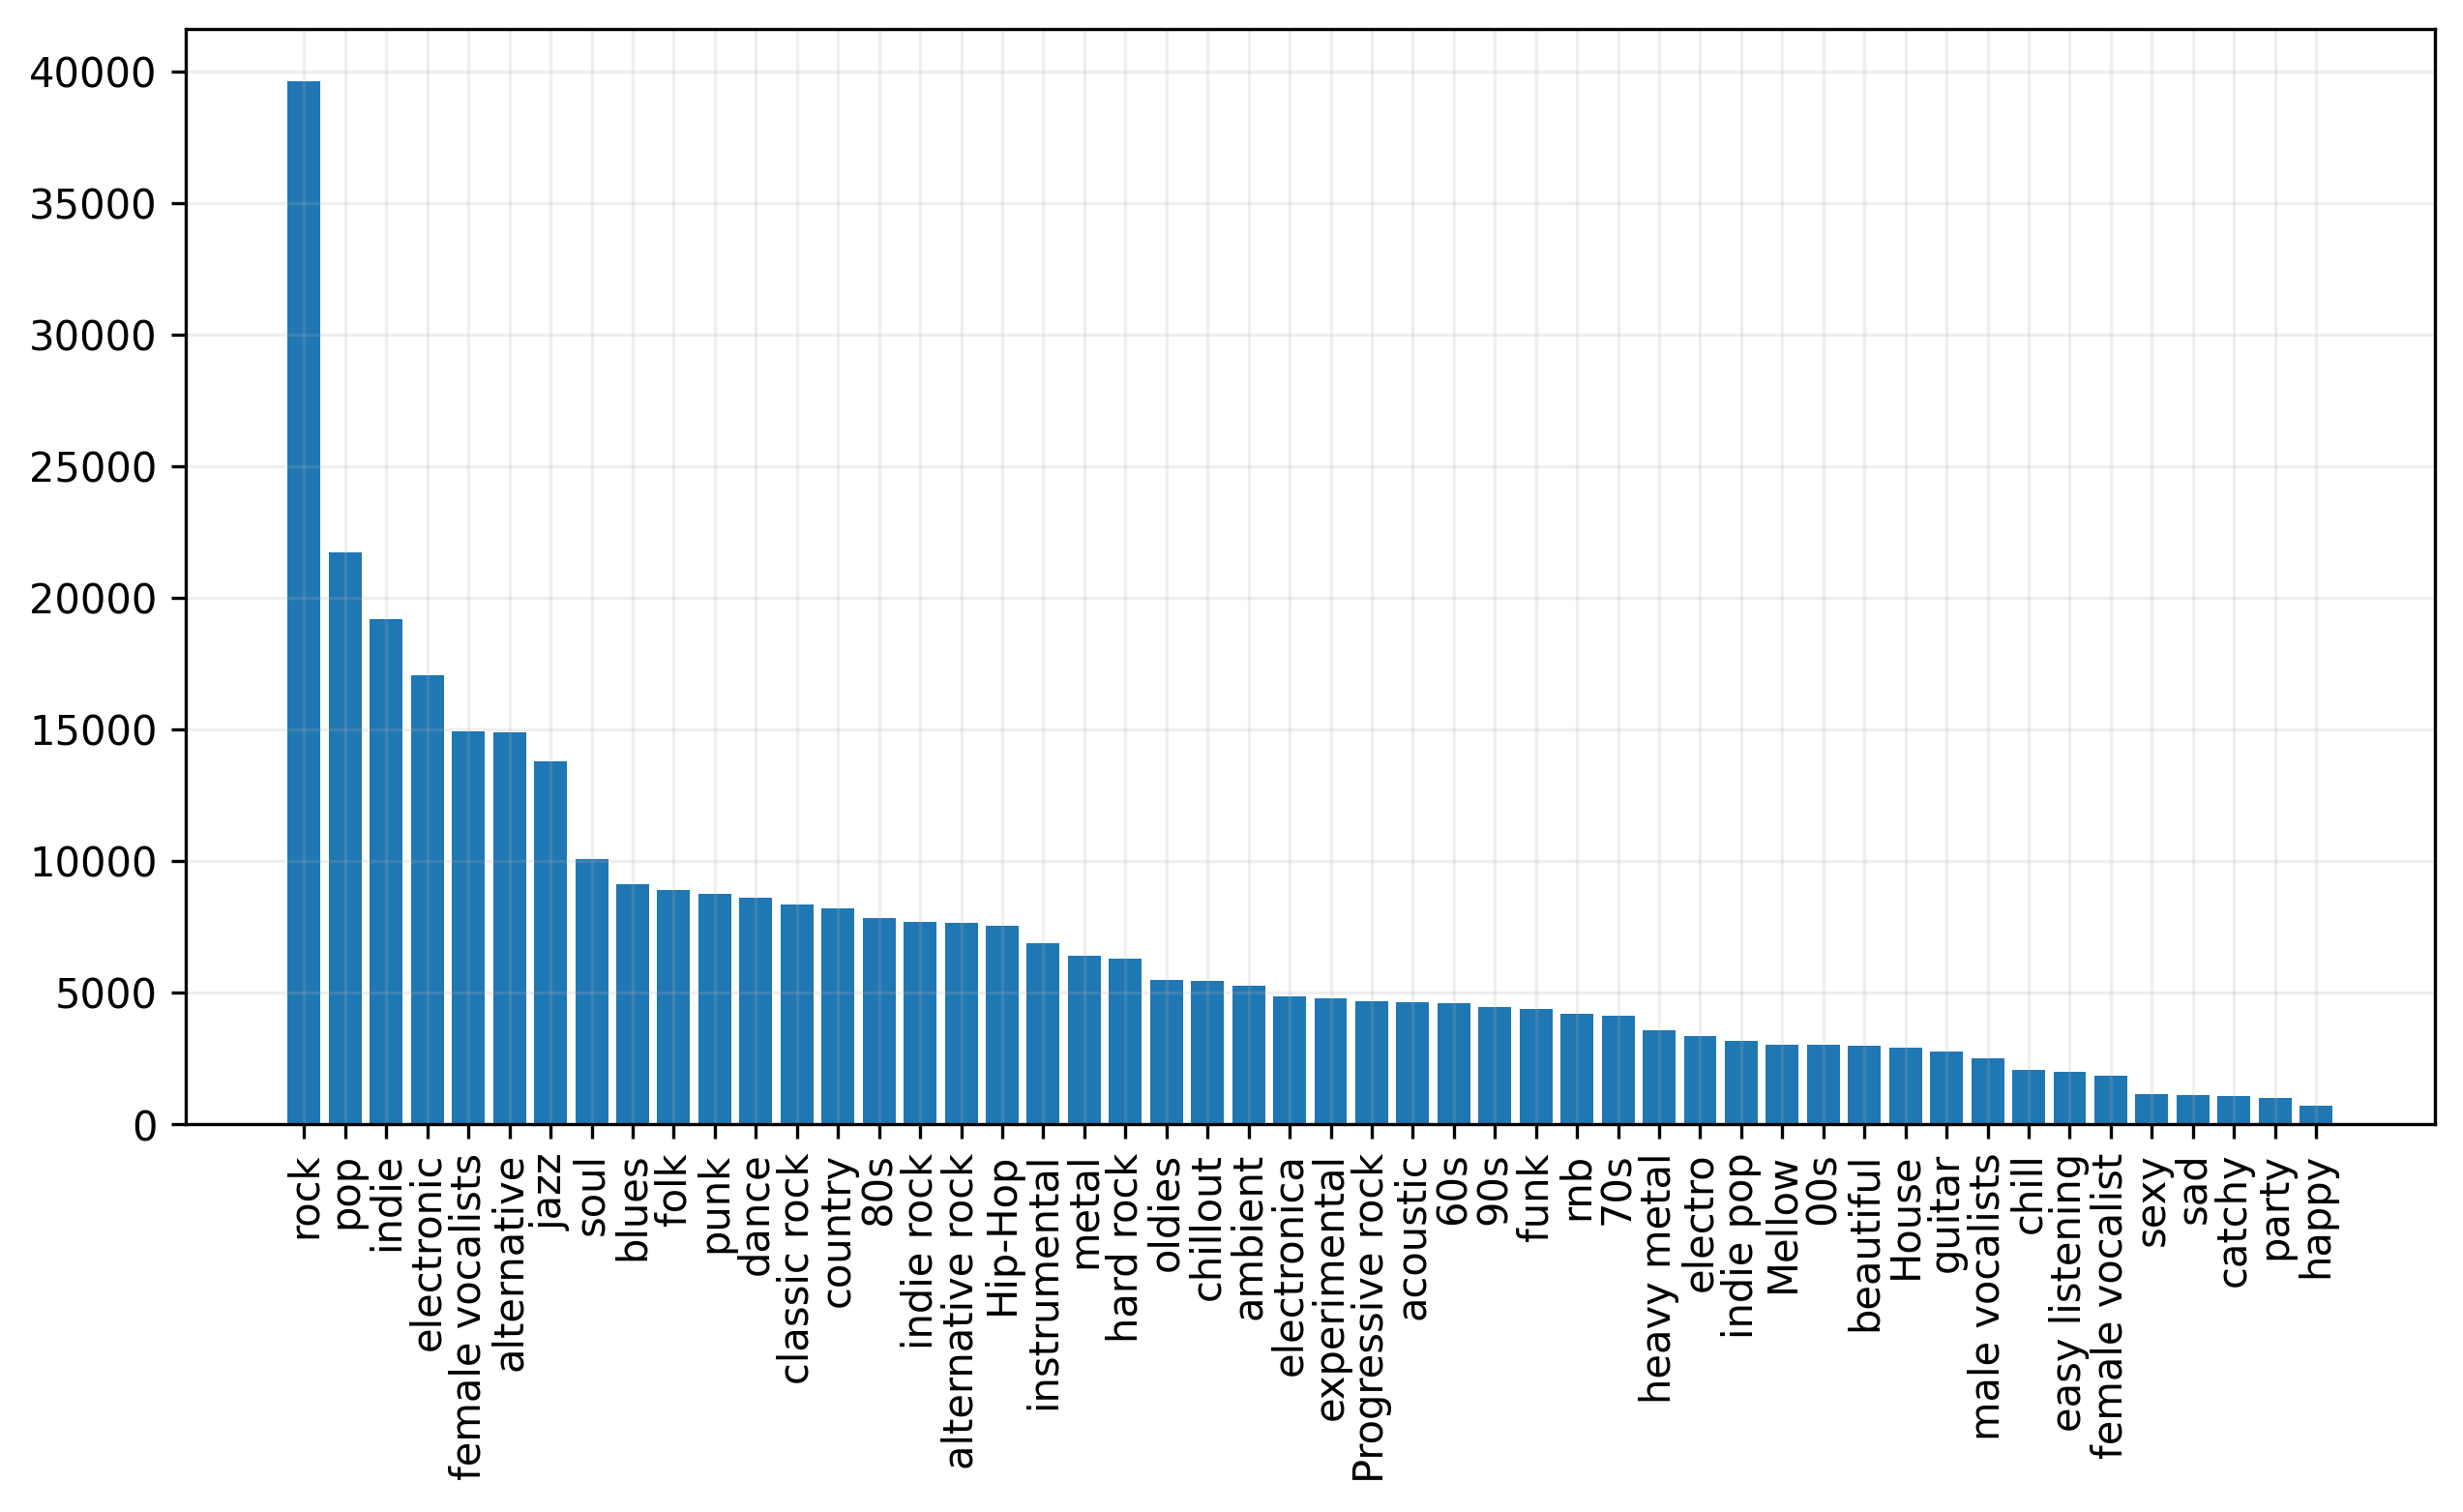
\includegraphics[width=\columnwidth]{figs/tag_stats_msd.png}
    \caption{Distribution of tags of the Million Song Dataset}
    \label{fig:tag_stats_msd}
\end{figure}


\begin{table}[t]
    \centering
    \begin{tabular}{lll}\toprule
        rock & pop & alternative \\
        indie & electronic & female vocalists \\
        dance & 00s & alternative rock \\
        jazz & beautiful & metal \\
        chillout & male vocalists & classic rock \\
        soul & indie rock & mellow \\
        electronica & 80s & folk \\
        90s & chill & instrumental \\
        punk & oldies & blues \\
        hard rock & ambient & acoustic \\
        experimental & female vocalist & guitar \\
        hip-hop & 70s & party \\
        country & easy listening & sexy \\
        catch & funk & electro \\
        heavy metal & progressive rock & 60s \\
        rnb & indie pop & sad \\
        house & happy & - \\
        \bottomrule
    \end{tabular}
    \caption{50 most popular tags in the Million Song Dataset}
    \label{tab:msd_tags}
\end{table}




\section{Transfer Learning datasets}

\subsection{McGill Billboard Dataset}
\subsection{GTZAN}


